\begin{frame}{Finer grained parallelism for GPUs, low order}
%\begin{figure}
\centering
\tikzstyle{work group} = [draw,green,rounded corners]
\tikzstyle{thread}     = [fill,red]
\tikzstyle{operation}  = [dashed,rounded corners]
\tikzstyle{notation}   = [anchor=south,text width=4cm,text centered]
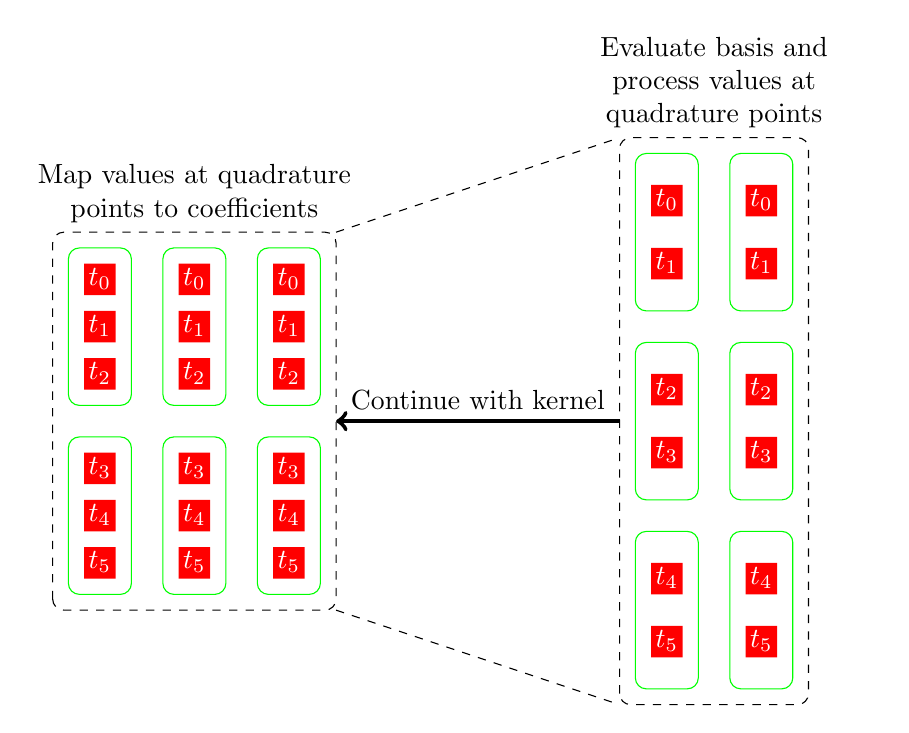
\begin{tikzpicture}[scale=0.4]
% Draw the basis function evaluation
\draw[operation] (-0.5,-0.5) rectangle +(9,12)
  ++(4.5,12) node[notation] {Map values at quadrature points to coefficients};
% Draw the basis function evaluation breakdown
\foreach \x in {0, 3, 6}
  \foreach \y/\j in {0/1, 6/0}
{
  % draw a cell work unit
  \path[work group] (\x,\y) rectangle +(2,5);
  % draw a 3 thread configuration
 \path[thread] (\x,\y)
             ++(0.5,0.5)
              +(0,0) rectangle +(1,1) +(0.5,0.5) node[anchor=mid,text=white] {\pgfmathtruncatemacro{\t}{\j*3+2}$t_{\t}$}
             ++(0.0,1.5)
              +(0,0) rectangle +(1,1) +(0.5,0.5) node[anchor=mid,text=white] {\pgfmathtruncatemacro{\t}{\j*3+1}$t_{\t}$}
             ++(0.0,1.5)
              +(0,0) rectangle +(1,1) +(0.5,0.5) node[anchor=mid,text=white] {\pgfmathtruncatemacro{\t}{\j*3+0}$t_{\t}$};
}
% Draw arrow for kernel continuation
\draw[<-,ultra thick] (8.5,5.5) -- node[anchor=south] {Continue with kernel} (17.5,5.5);
\draw[dashed] (8.5,11.5) -- (17.5,14.5);
\draw[dashed] (8.5,-0.5) -- (17.5,-3.5);
% Draw the quadrature point evaluation
\draw[operation] (17.5,-3.5) rectangle +(6,18)
  ++(3,18) node[notation] {Evaluate basis and process values at quadrature points};
% Draw the quadrature point evaluation breakdown
\foreach \x in {18, 21}
  \foreach \y/\j in {-3/2, 3/1, 9/0}
{
  % draw a cell work unit
  \path[work group] (\x,\y) rectangle +(2,5);
  % draw a 2 thread configuration
 \path[thread] (\x,\y)
             ++(0.5,1.0)
              +(0,0) rectangle +(1,1) +(0.5,0.5) node[anchor=mid,text=white] {\pgfmathtruncatemacro{\t}{\j*2+1}$t_{\t}$}
             ++(0.0,2.0)
              +(0,0) rectangle +(1,1) +(0.5,0.5) node[anchor=mid,text=white] {\pgfmathtruncatemacro{\t}{\j*2+0}$t_{\t}$};
}
\end{tikzpicture}
% \caption{Action of the residual evaluation kernel on a group of incoming cells. Each cell is displayed as a green,
%   rounded rectangle occupied by the threads which compute the cell information. Each thread computes its values in
%   series, so that thread $t_0$ first computes values at quadrature points for 2 cells, and then computes basis
%   coefficients for 3 cells.}
%\end{figure}
\end{frame}
